\documentclass{beamer}

\usepackage{mathptmx,wrapfig}
%\usepackage{helvet}
\mode<presentation>
{
  \usecolortheme{rose}
  \usecolortheme{dolphin}
  \setbeamercolor*{author in head/foot}{parent=palette secondary}
  \setbeamercolor*{title in head/foot}{parent=palette tertiary}
  \useinnertheme{rectangles}
  \setbeamertemplate{navigation symbols}{}
  \setbeamertemplate{footline}{
  \leavevmode%
  \hbox{%
  \begin{beamercolorbox}[wd=.5\paperwidth,ht=2.25ex,dp=1ex,center]{author in head/foot}%
    \usebeamerfont{author in head/foot}\insertshortauthor~~\insertshortinstitute
  \end{beamercolorbox}%
  \begin{beamercolorbox}[wd=.5\paperwidth,ht=2.25ex,dp=1ex,center]{title in head/foot}%
    \usebeamerfont{title in head/foot}\insertshorttitle
  \end{beamercolorbox}}%
  \vskip0pt%
  }
  \setbeamertemplate{frametitle}[default][center]
}

\date{}

\usepackage[english]{babel}
\usepackage{epsfig}
\usepackage{hyperref}
\usepackage{graphicx}
\usepackage{amsthm}
\usepackage{amsmath}
\usepackage{amsfonts}
\usepackage{amssymb}
\usepackage{listings}
%\input{psfig.sty}

\newcommand{\ip}[2]{\langle #1,#2 \rangle}
\newtheorem{result}{Result}

\title{Large Scale Optimization: Lecture 16}
\author{Fall 2014}
\institute[]{The University of Texas at Austin}

\begin{document}

\begin{frame}
  \titlepage
\end{frame}

%%%%%%%%%%%%%%%%%%%%%%%%%%%%%%%%%%%%%%%%%%%%%%%%%%%%%%%%%%%%%%%%%%
\begin{frame}
  \frametitle{Recap}
  \begin{itemize}
      \item Dual of {\it Semi-Definite Programming (SDP)} problems with linear
objective function are derived as 
\begin{equation}
\begin{aligned}
    &\underset{}{\text{min}} && - \langle G, Z \rangle  \\
    &\text{ s.t.} && \langle F_i, Z \rangle = c_i,\ \forall i  \\
       & && z \succeq 0
\end{aligned}
\end{equation}
\item Application of linear SDP optimization:
\begin{itemize}
    \item Find a matrix with largest eigenvalue, 
    \item Find sum of $r$-largest eigenvalues of a given matrix and
    \item Find sum of singular values of a symmetric but not PSD matrix.
\end{itemize}
\end{itemize}
\end{frame}

%%%%%%%%%%%%%%%%%%%%%%%%%%%%%%%%%%%%%%%%%%%%%%%%%%%%%%%%%%%%%%%%%%
\begin{frame}
\frametitle{Recap}
\begin{itemize}
    \item Study of SDP is then extended to non-linear objective, called
{\it Log Determinant Optimization}. The general form is as follows:
\begin{equation}
\begin{aligned}
    &\underset{x}{\text{min }} && c^T x - \text{log det } G(x) \\
    &\text{ s.t.} && G(x) \succeq 0 \\
    & && F(x) \geq 0
\end{aligned}
\end{equation}
where $- \text{log det } G(x)$ is proven to be convex function. 
\end{itemize}
\end{frame}

%%%%%%%%%%%%%%%%%%%%%%%%%%%%%%%%%%%%%%%%%%%%%%%%%%%%%%%%%%%%%%%%%%
\begin{frame}
\frametitle{Recap}
\begin{itemize}
\item Following problems are formulated as Log Determinant Optimization
problem:
\begin{itemize}
    \item Find the minimal-volume ellipsoid that contains all given points, 
    \item Find the maximum-volume ellipsoid enclosed within a given polyhedron, 
    \item Find the most likely parameters that generates a given set of samples
    \item Find the variance matrix of gaussian channel with maximum capacity.
\end{itemize}
\end{itemize}

\end{frame}

%%%%%%%%%%%%%%%%%%%%%%%%%%%%%%%%%%%%%%%%%%%%%%%%%%%%%%%%%%%%%%%%%%
\begin{frame}
\frametitle{Motivations for Proximal Gradient Descent}
\begin{itemize}
    \item Motivation 1: Iterative Shrinkage-Thresholding Algorithm (ISTA)
    \item Motivation 2
\end{itemize}
\end{frame}

%%%%%%%%%%%%%%%%%%%%%%%%%%%%%%%%%%%%%%%%%%%%%%%%%%%%%%%%%%%%%%%%%%
\begin{frame}
\frametitle{Iterative Shrinkage-Thresholding Algorithm (ISTA)}
Consider the unconstrained optimization problem with $l_1$ regularization
\begin{equation}
\begin{aligned}
    & \underset{x}{\text{ min }}
    && \frac{1}{2}\underbrace{|| y - Ax ||_2^2}_{\text{smooth/"nice"}}
    + \underbrace{  \lambda || x ||_1 }_{\text{not smooth/"nice", but "special"}}
\end{aligned}
\end{equation}
If $A = I$, then
\begin{equation}
\begin{aligned}
    & \underset{x}{\text{ min }} 
    && \frac{1}{2} || y - x ||_2^2 + \lambda || x ||_1 \\
    = 
    & \underset{x}{\text{ min }} 
    && \sum_i \{ \frac{1}{2} ( y_i - x_i )^2  + \lambda | x_i |_1 \} \\
\end{aligned}
\end{equation}
\end{frame}

%%%%%%%%%%%%%%%%%%%%%%%%%%%%%%%%%%%%%%%%%%%%%%%%%%%%%%%%%%%%%%%%%%
\begin{frame}
\frametitle{Iterative Shrinkage-Thresholding Algorithm (ISTA)}
Now we derive closed-form solution for each "separated" problem: 
\begin{align}
    x_i-y_i + \lambda & && \text{ if } x_i > 0 \\
    x_i-y_i - \lambda & && \text{ if } x_i < 0 \\
    -y_i + r \lambda &, r \in (-1,1) && \text{ if } x_i = 0 
\end{align}
Suppose $y_i > 0$, then it obvious that $x_i \geq 0 $. 
\begin{itemize}
    \item if $x_i > 0$, then $\exists x_i = y_i - \lambda$.
    \item if $x_i = 0$, then 
\end{itemize}
Similarly, if $y_i < 0$, then exists $x_i = y_i + \lambda$ if $x_i < 0$.
% TODO: add figure here
\end{frame}

%%%%%%%%%%%%%%%%%%%%%%%%%%%%%%%%%%%%%%%%%%%%%%%%%%%%%%%%%%%%%%%%%%
\begin{frame}
\frametitle{Motivation 2}
Consider another optimization problem
\begin{equation}
\begin{aligned}
    &  \underset{x}{\text{ min }}
    && \underbrace{g(x)}_{\text{"nice"}} \\
    &  \text{ s.t. } 
    && x \in Q
\end{aligned}
\end{equation}
where $Q$ is a convex set and is easy to project onto, e.g. $Q: \{ x| ||x||_{\infty} \leq 1 \}$. \\
The above optimization problem equates to 
\begin{equation}
\begin{aligned}
    &  \underset{x}{\text{ min }}
    && g(x) + I_Q(x) 
\end{aligned}
\end{equation}
where 
\begin{equation}
    I_Q (x) = 
   \begin{cases}
   0 &\mbox{if } x \in Q  \\
   \infty &\mbox{if } x \not \in Q
   \end{cases}
  \end{equation}
Hence, we have 
\begin{equation}
    [P_Q(y)]_i =
   \begin{cases}
   y_i &\mbox{if } |y_i| \leq 1  \\
   sign(y_i) &\mbox{otherwise} 
   \end{cases}
  \end{equation}

\end{frame}

%%%%%%%%%%%%%%%%%%%%%%%%%%%%%%%%%%%%%%%%%%%%%%%%%%%%%%%%%%%%%%%%%%

\begin{frame}
\frametitle{Proximal Gradient Algorithm}
\begin{itemize}
\item Unconstrained problem with sum of two functions:
\begin{equation}
\textrm{minimize}~f(x)=g(x)+h(x)
\end{equation}
\vspace{-2.5em}
\begin{align*}
g(x)&: \textit{'nice'}, \text{ (ex) convex, L-lipschitz gradient}\\
h(x)&: \textit{'special'}, \text{ (ex) convex, not smooth, \textbf{prox} is inexpensive}
\end{align*}
\end{itemize}
\begin{definition}
\textbf{\em{- Prox function/ Proximal operator}}\\
The prox function (or proximal operator) of a function $h(\cdot)$ is defined as:
\begin{equation}
\textbf{prox}_{th}(v) = \arg\min_{x} \left( h(x)+\frac{1}{2t}\|x-v\|_2^2 \right)
\end{equation}
\end{definition}

\end{frame}

\begin{frame}
\frametitle{Prox function/ Proximal operator}
\begin{columns}
\column{0.45\linewidth}
\centering
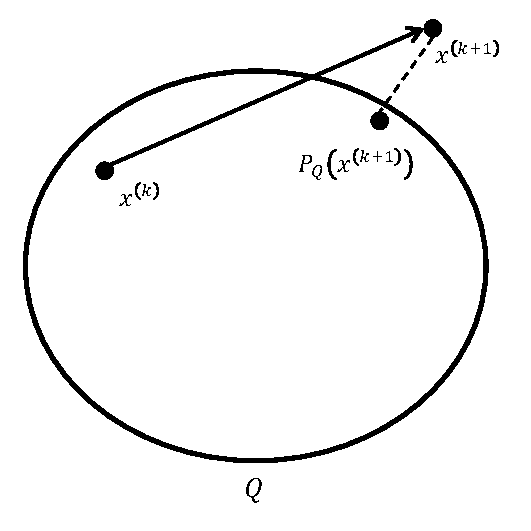
\includegraphics[scale=0.5]{L16_fig_projection}
\column{0.5\linewidth}
\begin{itemize}
\item Ex) Projection on set $Q$
\end{itemize}
\begin{align*}
x^{(k+1)} &= P_Q \left( x^{(k)}-t \nabla g(x^{(k)})\right)\\
\textbf{prox}_h (x) &= \arg\min_u \left( I_Q (u) + \frac{1}{2}\|u-x\|_2^2 \right)\\
&= \arg\min_{u \in Q} \left( \frac{1}{2}\|u-x\|_2^2 \right)\\
&= P_Q (x)\\
I_Q (x) &=  \begin{cases}
	0 & \text{if}~x \in Q \\
	\infty & \text{if}~x \notin Q
	\end{cases}
\end{align*}
\end{columns} 

\end{frame}

\begin{frame}
\frametitle{Proximal Gradient Algorithm}
\noindent\textbf{- Proximal Gradient Algorithm}\\
\begin{equation*}
x_+ \leftarrow \textbf{prox}_{th} \left(x - t\nabla g(x) \right)
\end{equation*}
\begin{itemize}
\item Uses two black boxes for the task:\\
\centering minimize $f(x) = g(x) + h(x)$
\end{itemize}
\begin{figure}[ht]
    \centering
    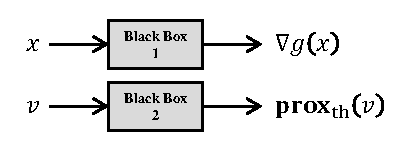
\includegraphics[scale=0.9]{L16_fig_twoblackboxes}\\
    \caption{Using two black boxes for proximal gradient}\label{16fig:twoblackboxes}
\end{figure}
\end{frame}

\begin{frame}
\frametitle{Proximal Gradient Algorithm}
\begin{itemize}
\item Form of quadratic approximation of $g(u)$ around $x$
\end{itemize}
\begin{align}
x_+ \leftarrow &\textbf{prox}_{th} \left(x - t\nabla g(x) \right)\nonumber\\
&= \arg\min_u \left( h(u)+\frac{1}{2t}\|u-x+t\nabla g(x)\|_2^2 \right)\nonumber\\
&= \arg\min_u \left( h(u)+\langle \nabla g(x), u-x \rangle + \frac{1}{2t}\|u-x\|_2^2 +\frac{t}{2}\| \nabla g(x) \|_2^2 \right)\nonumber\\
&= \arg\min_u \left( h(u)+\langle \nabla g(x), u-x \rangle + \frac{1}{2t}\|u-x\|_2^2 + g(x) \right)
\end{align}\label{16eq:prox_quadratic}

\end{frame}

\begin{frame}
\frametitle{Convergence Analysis of Proximal Gradient}
\begin{theorem}\label{16thm:convergence}
If $g$ is convex and $g$ has L-lipschitz gradient, i.e. $\| \nabla g(x) - \nabla g(y)\|_2 \leq L\|x-y\|_2$, using fixed size $t < 1/L$ on proximal gradient algorithm gives $O(1/\epsilon)$ of convergence to the optimal point $x^*$, where $x^* = \arg\min_x \left( g(x) + h(x)\right)$.
\end{theorem}
\begin{itemize}
\item Introducing $G_t(x)$
\end{itemize}
\vspace{-1em}
\begin{align*}
x_+ \leftarrow x-t G_t (x)&=\textbf{prox}_{th}(x-t\nabla g(x))\\
\Leftrightarrow G_t (x) &\triangleq \frac{1}{t}\left( x - \textbf{prox}_{th}(x-t\nabla g(x)) \right)
\end{align*}
\end{frame}

\begin{frame}
\frametitle{Convergence Analysis of Proximal Gradient\\- Preliminaries for proof}
\begin{block}{Claim}
$G_t (x)- \nabla g(x) \in \partial h(x-tG_t (x))$
\end{block}
\begin{lemma}
\label{16lemma:quadratic} 
For any point $z$, $f(x_+)\leq f(z)+ \langle G_t (x),x-z \rangle -\frac{t}{2}\|G_t (x)\|_2^2 $
\end{lemma}
Proof of Claim and Lemma: Later

\end{frame}

\begin{frame}
\frametitle{Proof of Theorem}
Putting $z=x$ in the Lemma gives,
\begin{equation*}
f(x_+) \leq f(x)-\frac{t}{2}\|G_t (x)\|_2^2
\end{equation*}
This gives the decreasing property $f(x_+) \leq f(x)$\\
And putting $z=x^*$ gives,
\begin{align*}
f(x_+) &\leq f^*-\frac{t}{2}\|G_t (x)\|_2^2+\langle G_t (x),x-x^* \rangle\\
\Leftrightarrow f(x_+)-f^* &\leq \frac{1}{2t}\left[ \|x-x^* \|_2^2 - \|x-x^*-tG_t(x)\|_2^2 \right]\\
&=\frac{1}{2t}\left[ \|x-x^* \|_2^2 - \|x_+ -x^*\|_2^2 \right]
\end{align*}


\end{frame}

\begin{frame}
\frametitle{Proof of Theorem}
Adding up over $T$ iterations gives
\begin{align*}
\sum_{k=1}^{T}\left(f(x^{(k)})-f^* \right) &\leq \frac{1}{2t} \left[\|x^{(0)}-x^*\|_2^2 - \|x^{(T)}-x^*\|_2^2\right] \\
&\leq \frac{1}{2t}\|x^{(0)}-x^*\|_2^2
\end{align*}
From the fact that $f(x_+) \leq f(x)$,
\begin{equation*}
f(x^{(k)})-f^* \geq f(x^{(T)})-f^* \text{ for } k=1,\cdots T
\end{equation*}
This gives,
\begin{equation*}
f(x^{(T)})-f^* \leq \frac{1}{2tT} \|x^{(0)}-x^*\|_2^2
\end{equation*}
$\Rightarrow~ O(1/\epsilon)$ convergence\\
(requires $k= O(1/\epsilon)$ of iteration number for $f(x^{(k)})-f^* \leq \epsilon$)

\end{frame}

\begin{frame}
\frametitle{Proof of Lemma}
From the L-lipschitz continuous of gradient on $g$,
\begin{equation*}
g(y) \leq g(x) + \langle \nabla g(x),y-x \rangle +\frac{L}{2}\|y-x\|_2^2
\end{equation*}
So, for $y=x_+=x-tG_t(x)$
\begin{equation}\label{16eq:lemma_proof1}
g(x_+) \leq g(x)- \langle \nabla g(x), tG_t(x) \rangle +\frac{L}{2}t^2 \|G_t(x)\|_2^2
\end{equation}
Recall the definition of subgradient,
\begin{equation*}
a \in \partial h(x_+) \Longleftrightarrow h(z) \geq h(x_+)+\langle a,z-x_+ \rangle
\end{equation*}
By Claim, $G_t(x)-\nabla g(x) \in \partial h(x-tG_t(x))$
\begin{align}
h(z) &\geq h(x_+) + \langle G_t(x) -\nabla g(x),z-x_+ \rangle \nonumber\\
\Leftrightarrow ~h(x_+)&\leq h(z)-\langle G_t(x) -\nabla g(x),z-x_+ \rangle
\label{16eq:lemma_proof2}
\end{align}
\end{frame}

\begin{frame}
\frametitle{Proof of Lemma}
Add (\ref{16eq:lemma_proof1}), (\ref{16eq:lemma_proof2}) and use $f(x_+)=g(x_+)+h(x_+)$
\begin{align*}
f(x_+) \leq ~&g(x)- \langle \nabla g(x), tG_t(x) \rangle +\frac{L}{2}t^2 \|G_t(x)\|_2^2\\
&+h(z)-\langle G_t(x) -\nabla g(x),z-x_+ \rangle\\
\leq ~&g(z) -\langle \nabla g(x),z-x \rangle - \langle \nabla g(x), tG_t(x) \rangle +\frac{L}{2}t^2 \|G_t(x)\|_2^2\\
&+h(z)-\langle G_t(x) -\nabla g(x),z-x_+ \rangle \\
&\hspace{2em}(\because g(x) \leq g(z)-\langle \nabla g(x),z-x \rangle \text{ from convexity of } g)\\
= ~&f(z)+\frac{L}{2}t^2 \|G_t(x)\|_2^2 - \langle G_t(x),z-x+tG_t(x) \rangle\\
\leq ~&f(z)+\langle G_t (x),x-z \rangle+\frac{t}{2}\|G_t(x)\|_2^2-t \|G_t(x)\|_2^2 \hspace{1em}(\because t<1/L)\\
= ~&f(z)+\langle G_t (x),x-z \rangle-\frac{t}{2}\|G_t(x)\|_2^2
\end{align*}
\end{frame}

\begin{frame}
\frametitle{Proof of Claim}
\textbf{Claim}. $G_t(x)-\nabla g(x) \in \partial h(x_+)$\\
\begin{itemize}
\item Property of proximal operator\\
\begin{equation}\label{16eq:claim1_sub}
u=\textbf{prox}_{th}(x) \Leftrightarrow \frac{1}{t}(x-u) \in \partial h(u)
\end{equation}
(Proof: Use that $\textbf{prox}_{th}(x)$ is a minimizer)
\end{itemize}
\vspace{1em}
Now put $u=x_+ = \textbf{prox}_{th}(x-\nabla g(x))$ in equation (\ref{16eq:claim1_sub}),
\begin{align*}
\Rightarrow ~&\frac{1}{t}(x-\nabla g(x) - x_+) \in \partial h(x_+)\\
\Rightarrow ~&\frac{1}{t}(x-\nabla g(x) - x+tG_t(x)) \in \partial h(x_+)\\
\Rightarrow ~&G_t(x) -\nabla g(x) \in \partial h(x_+)
\end{align*}
\end{frame}

\begin{frame}
\frametitle{Next lecture}
\begin{itemize}
\item Review of oracle complexity of algorithm
\item Nesterov's accelerated gradient descent
\end{itemize}
\vspace{2pc}
\center Thank you!
\end{frame}

\end{document}
